\chapter{Les Progiciels de Gestion Internes}

\section{Introduction}
Le but de ce chapitre est de présenter globalement le progiciel de gestion interne aussi appeler \acs{ERP}.\\

Dans un premier temps, nous définirons le concept d'\acs{ERP} et son évolution dans le temps.\\

Par la suite, nous aborderons les avantages liés a l'intégration d'un tel système dans les deux aspects administratif et opérationnel ainsi que ses inconvénients.\\

Nous finirons avec les multiples fonctionnalités de l'\acs{ERP}.\\

\section{Définition}
Le sigle \acs{ERP} veut dire Entreprise Resource Planning son semblable en Français est Progiciel de Gestion Intégré abrévié PGI.\\

Contrairement au MRP qui se contente de la planification des besoins, l’\acs{ERP} est un logiciel qui permet la gestion de l’ensemble des sous-systèmes d’une entreprise ainsi que la coordination de ceux-ci.\\

Pour y parvenir l’\acs{ERP} intègre l’ensemble des fonctions utiles d’une entreprise sous forme de modules qui partagent une base de données unique, ceci permet l’échange d’informations entre les modules, dans ce cas-là on parle de moteur de Workflow.

\section{Historique}
La création de l’\acs{ERP} revient principalement à Joseph Orlicky qui créa dans les années 1960 le MRP abréviation de Material Requirements Planning ancêtre de l’\acs{ERP}, le MRP répond essentiellement aux besoins de planification des entreprises.\\

La notion d’\acs{ERP} tel que nous la connaissons à fait son apparition dans les années 90, mais n’a connu son essor que dans les années 2000 avec l’arrivée de l’internet, l’utilisation de l’\acs{ERP} se généralise et évolue jusqu’à arriver à l’\acs{ERP} tel que nous le connaissons aujourd’hui.

\section{Avantages liés à l’intégration d’un \acs{ERP}}
Les bénéfices liés à l’implémentation d’un ERP ont été prouvé par bon nombre de recherches, l’une d’elles mener par le groupe Aberdeen qui ont quantifié et publié les résultats suivants :\\

\begin{itemize}
    \item Réduction des coûts d’opérations de 22\%
    \item Réduction des coûts d’administration de 20\%
    \item Réduction d’inventaires de 17\%
    \item Amélioration du temps de livraison de 19\%
    \item Amélioration du respect des délais et des budgets de 17\%\\
\end{itemize}

Même les entreprises en difficulté ont réalisé des bénéficies grâce à l’intégration de leur ERP, leurs résultats s’élèvent à :\\

\begin{itemize}
    \item Réduction des coûts d’opérations de 7\%
    \item Réduction des coûts d’administration de 4\%
    \item Réduction d’inventaires de 9\%
    \item Amélioration du temps de livraison de 11\%
    \item Amélioration du respect des délais et des budgets de 6\%\\
\end{itemize}

Comme l’étude le souligne le gain en pourcentage ne paraît pas impressionnant, mais pour chaque million de dollars déboursé dans les coûts d’opérations, 70 000 \$ sont économisé.\\

En effet nous pouvons constater les gains en productivité et en maturité des entreprises, pour y parvenir l’\acs{ERP} procède à une amélioration sur plusieurs aspects :

\subsection{Aspect administratif}
En fusionnant tous les systèmes de l’entreprise en une seule application, l’installation de l’\acs{ERP} conduit à une réduction des coûts d’exploitation et de maintenance, et comme l’\acs{ERP} possède une architecture sous forme modulaire il fournit une infrastructure qui assure une flexibilité en cas de changements futurs, donc offre la possibilité d’implémenter de nouvelles fonctionnalités.\\

Une seule application donc une seule base de données, cette base de données unique permet un gain de temps. Réduire le volume d’information inutile et d’éviter les saisies multiples, donc l’installation de l’\acs{ERP} permet la résolution des problèmes d’incohérence des informations et rend les données enregistrées plus fiables.\\

De plus cela évite les activités manuelles de traitement, de comparaison et de recherche réaliser par les employés dans le cadre de l’interfaçage des différents services. Ce qui conduit à un gain de temps et une croissance de la productivité administrative.

\subsection{Aspect opérationnel}
L’utilisation d’un \acs{ERP} conduit à la suppression des risques opérationnels et aux risques de pertes liés à des erreurs humaines où des dysfonctionnements dans le contrôle interne, fraudes qui peuvent résulter d’un dysfonctionnement des systèmes d’information déjà en place, l’\acs{ERP} permet la pertinence des informations partagées et évite ces dysfonctionnements qui peuvent être plus ou moins grave et qui peuvent entrainer des coûts supplémentaires inutile.\\

L’\acs{ERP} permet aussi un suivie au niveau des achats jusqu’aux ventes. En effet, dès la création de la commande, des données telles que le calcul des marges et des crédits est généré automatiquement de façon dynamique réalisant ainsi une intégration financière, grâce à cette fonctionnalité, l’\acs{ERP} aide les dirigeants dans la planification et la prise de décision, et leur permet d’améliorer la gestion des ressources, et ainsi améliorer les décisions opérationnelles.\\

De plus la centralisation est très bénéfique pour les services de finance. Car ce logiciel permet également la centralisation des tâches qui permet à une amélioration de la productivité en réduisant le nombre du personnel qui travaille sur la même tâche, cela permet des économies d’échelles notamment en matière de facturation.

\section{Inconvénients}
L’ERP offre des avantages non négligeables, mais une telle solution doit forcément comporter quelques désavantages.\\

Les projets ERP conduisent généralement à des coûts lors de la mise en place et de la maintenance. De plus la complexité des programmes utilisés requiert l’utilisation et l’entretien de serveurs puissants. Ce qui implique que le coût est souvent dépassé comme le montre l’étude CXP 2017.\\

\begin{figure}[H]
    \centering
    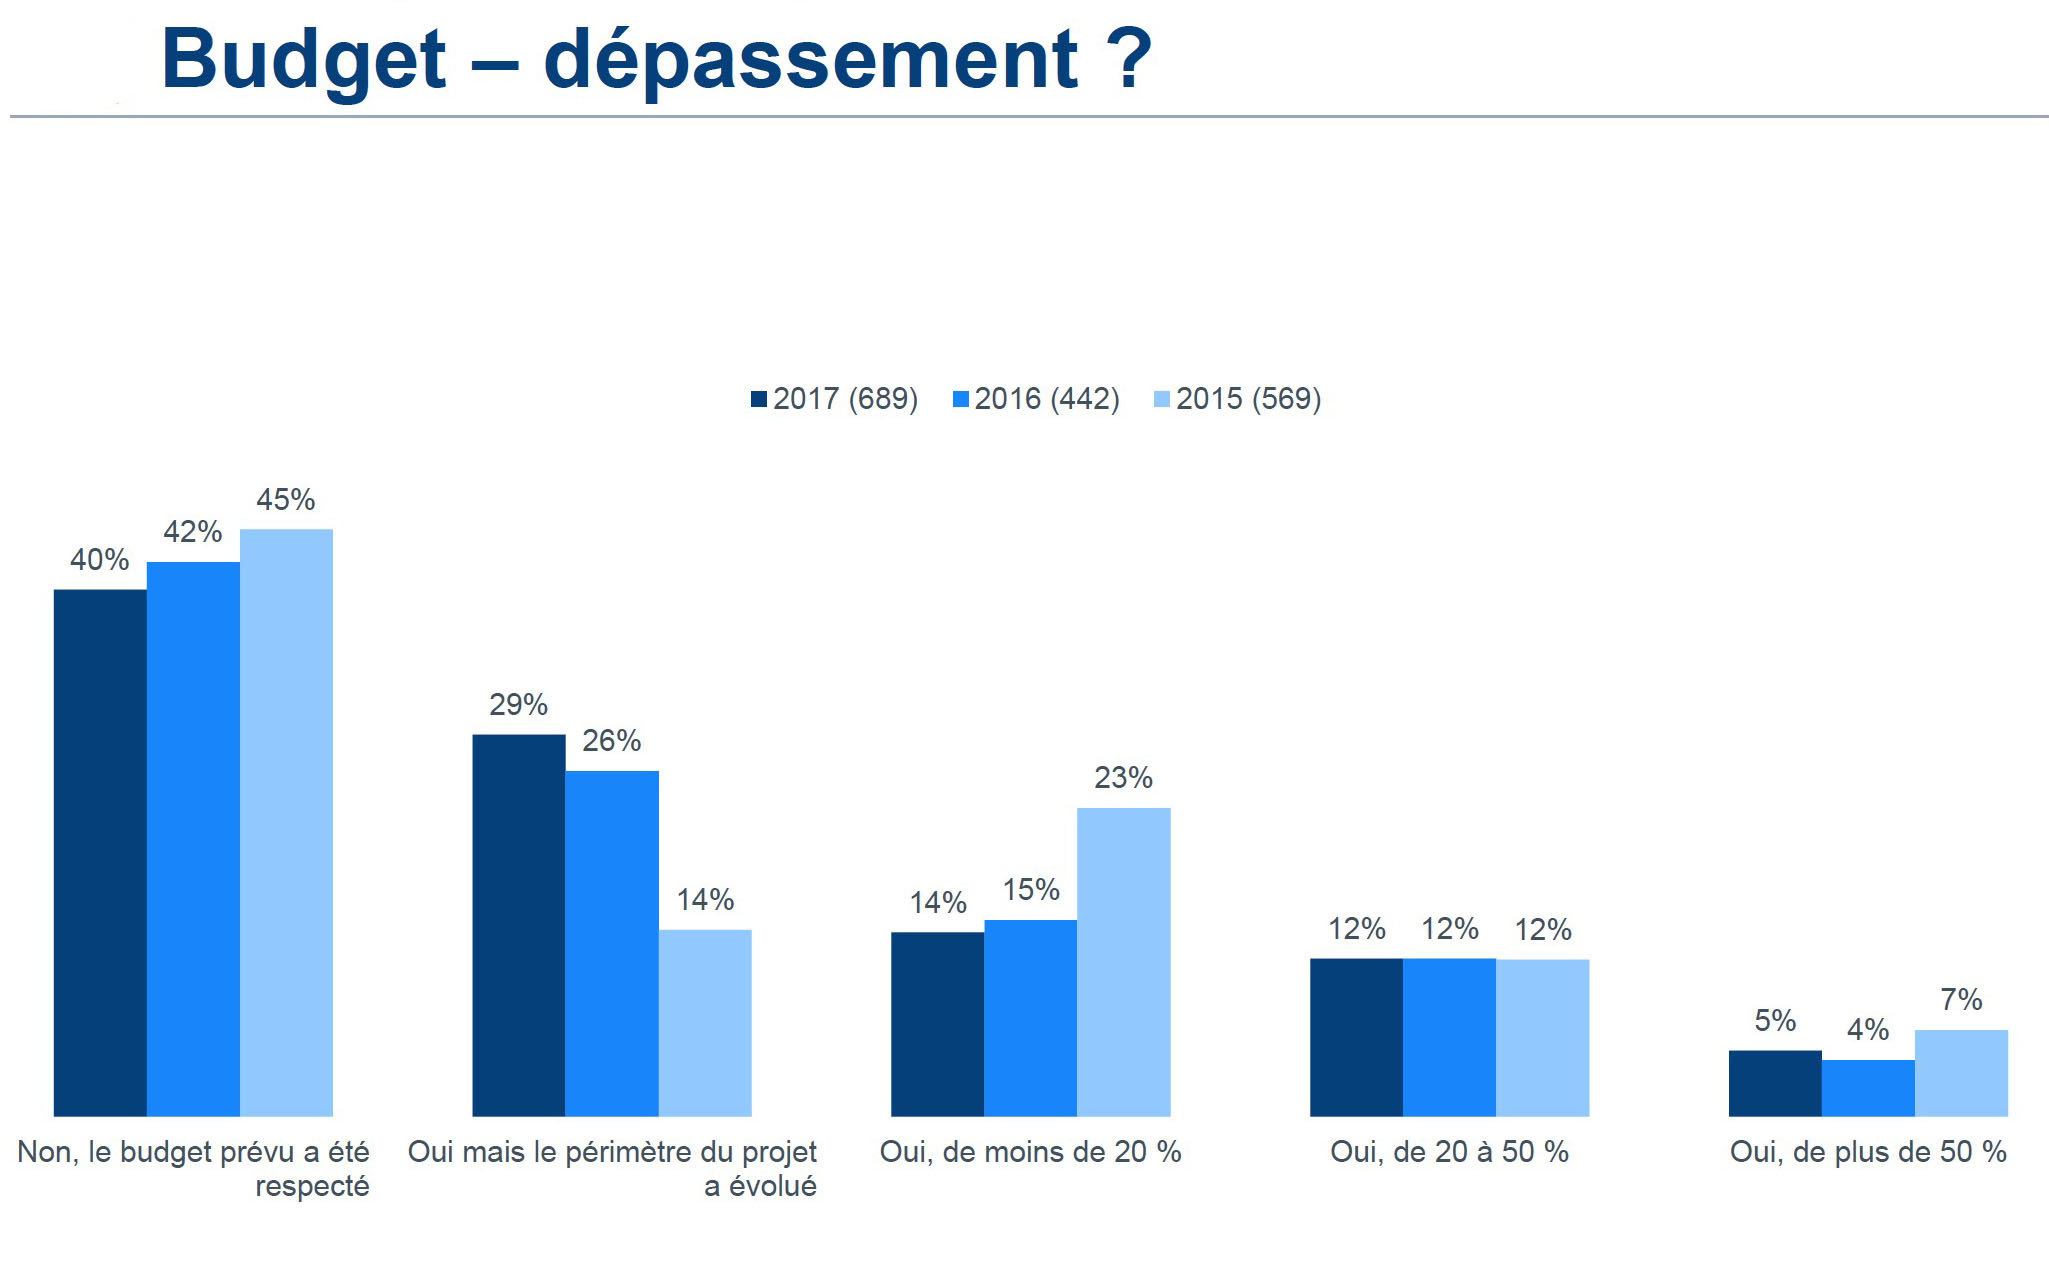
\includegraphics[scale=0.4]{ERP/graph-depassement-budget.jpg}
    \caption{Taux du dépassement de budget lors de l’implémentation d’un ERP}
\end{figure} 

On peut constater qu’en 2017 plus de 60\% des entreprises qui ont implémenté un ERP ont dépassé le budget prévu, 58\% en 2016 et 55\% en 2015.\\

En outre du coût, un projet de cette envergure requiert un temps et des ressources qui peuvent dépasser les prévisions, tel que le montre l’étude ERP Report 2010 du cabinet de conseil Panorama Consulting.\\

\begin{figure}[H]
    \centering
    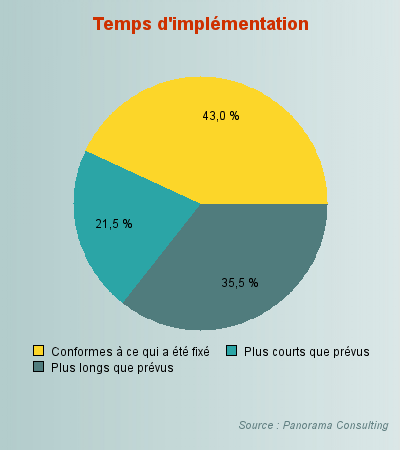
\includegraphics[scale=0.65]{ERP/graph-taux-implementation.png}
    \caption{Taux des dépassements des délais lors de l’implémentation d’un ERP}
\end{figure} 

Cette étude montre que plus de 35.5\% des entreprises ayant mis en place un ERP, ont vu le temps prévu pour l’implémentation dépassée, il est aussi à noter que la durée moyenne de la mise en place d’un ERP est de 18,4 mois qui varient d’un éditeur à un autre.

\section{Fonctionnalités}
L’ERP gère et organise les informations de l’ensemble des services de l’entreprise de façon automatique et dynamique, de l’achat des ressources à la vente en passant par la production, ces fonctionnalités sont nombreuses. Les modules plus couramment utilisés sont les suivants : \\

\begin{itemize}
    \item Gestion d’achats
    \item Gestion de la chaine logistique
    \item Gestion de stock et d’inventaire
    \item Gestion de production
    \item Gestion de projet
    \item Gestion des ressources humaines 
    \item Gestion comptabilité
    \item Gestion commerciale
    \item CRM : Gestion des relations clients\\
\end{itemize}

Chaque module couvre des fonctionnalités qui lui sont propres, dans le tableau ci-dessous une présentation de certains modules et des fonctionnalités qu’ils proposent.

\begin{table}[H]
    \begin{center}
        
        \begin{tabular}{|F{4cm}|R{10cm}|}
            \hline
            \textbf{Modules}  & \makecell[c]{\textbf{Fonctionnalités}} \\
            \hline
            Achats
            &
            Gestion de toutes les transactions comptables, telle que les bons de commande pour l’approvisionnement. Etc.\\
            
            \hline
            Chaine logistique
            &
            Gestion des ressources utilisées pour le pilotage de la chained’approvisionnement et de livraison.\\
            
            \hline
            Stock
            &
            Gestion des mouvements du stock, état du stock, entreposage.\\
            
            \hline
            Production
            &
            La gestion de la production, permet de réguler l’offre et les besoins en
            ressources par apport à la demande, impliquent la planification des ordres
            de fabrication et le contrôle de qualité.\\
            
            \hline
            Gestion de projet
            &
            Gestion de l’ensemble des projets de l’entreprise, de ces tâches et de ces plannings.\\
            
            \hline
            Ressources humaines
            &
            Gestion des ressources humaines et l’organisation de la rémunération des employés ainsi que des plannings de travail de ceux-ci.\\
            
            
            \hline
            Comptabilité
            &
            Gestion des obligations comptable auxquelles l’entreprise est soumise et suivie en temps réel de la santé financière de celle-ci, ainsi que de la gestion de facturation et des multidevises.\\
            
            \hline
            Commerciale
            &
            Gestion de l’aspect commerciale de l’entreprise, permet la gestion de l’ensemble des commandes clients et de leur facturation, permet aussi la réalisation de devis rapide et précise.\\
            
            \hline
            CRM
            &
            Gestion des relations clients, permet de réaliser de meilleurs suivis de
            l’environnement : clients, fournisseurs, prospects. etc.\\
            
            
            \hline
        \end{tabular}	
        \caption{Les Modules d'un ERP et leurs fonctionnalités}
    \end{center}
\end{table}

\section{Conclusion}
Après avoir défini lors de la première partie le concept d’entreprise, l’environnement et les contraintes auxquelles elle fait face. L’obligation de dégager un bénéfice est vitale, mais un certain nombre de points complexifient leurs systèmes d’information et freine la croissance économique de celle-ci, ces mêmes points qui rendent le recours à une technologie de l’information telle que l’ERP presque obligatoire.\\

Dans le deuxième point nous avons étudié l’ERP qui est au cœur du système d’information et qui permet la gestion de tous les services de l’entreprise. Ainsi que les avantages et les inconvénients à recourir à un tel outil.\\

Ensuite nous allons approfondir la recherche et étudier lors du deuxième chapitre, la gestion de stocks et d’approvisionnement.


\newpage

\leftskip=0cm
\renewcommand{\bibname}{Référence bibliographique et webographique du chapitre 1}
\bibliographystyle{ieeetr}	
\bibliography{ERP/erp}